\documentclass[a4paper]{report}
%%%%%%%% FONT %%%%%%%%
\usepackage[utf8]{inputenc}
\usepackage[T1,T2A,T5]{fontenc}
%%%%%%%% MATH %%%%%%%%
\usepackage{amsmath}
\usepackage{amsthm}
\usepackage{a4wide,amssymb,epsfig,latexsym,array,hhline,fancyhdr}
\usepackage[normalem]{ulem}
\usepackage[export]{adjustbox}
\usepackage{float}
%%%%%%%% CODE %%%%%%%%
\usepackage{listings}
%%%%%%%% COLOR %%%%%%%%
\usepackage{color}
\usepackage{xcolor, colortbl, rotating, multirow, booktabs, bigstrut}
\usepackage[makeroom]{cancel}
\usepackage{booktabs}
\usepackage{alltt}
\usepackage[framemethod=tikz]{mdframed}
\usepackage{caption,subcaption}
\usepackage{placeins}
\usepackage[lined,boxed,commentsnumbered]{algorithm2e}
\usepackage{enumerate}
%%%%%%%% GRAPHIC %%%%%%%%
\usepackage{graphicx}
\usepackage{graphics}
\usepackage{geometry}
\usepackage{tikz}
% \usetikzlibrary{arrows,snakes,backgrounds}
%%%%%%%% TABLE %%%%%%%%
\usepackage{multicol,longtable,amscd}
\usepackage{tabularx, caption}
\usepackage{multirow}
\usepackage{multicol}
\usepackage[export]{adjustbox}
%%%%%%%% FORMAT %%%%%%%%
\usepackage{lastpage}
\usepackage{array}
\usepackage{rotating}
\usepackage{setspace}
\usepackage{epsfig}
\usepackage{blindtext}
\usepackage{enumitem}
%%%%%%%% HYPERREF %%%%%%%%
\usepackage[unicode]{hyperref}
\hypersetup{urlcolor = blue,linkcolor=black,citecolor=black,colorlinks=true} 
\usepackage{tabularray}
\captionsetup[table]{name=Table}

%%%%%%%% DEFINE %%%%%%%%
\definecolor{BLUE}{rgb}{0.54,0.86,0.87}
\definecolor{ORANGE}{rgb}{0.99, 0.95, 0,96}
\definecolor{dkgreen}{rgb}{0,0.6,0}
\definecolor{gray}{rgb}{0.5,0.5,0.5}
\definecolor{backcolor}{rgb}{0.95,0.95,0.92}
%%%%%%%% BK THESIS %%%%%%%%
\usepackage{bkthesis}

\usepackage[normalem]{ulem}

\def\thesislayout{
    \geometry{
        a4paper,
        total={160mm,240mm}, 
        left=30mm,
        top=30mm,
    }
}
\thesislayout

\setlength{\headheight}{40pt}
\pagestyle{fancy}
\fancyhead{}
\fancyhead[L]{
 \begin{tabular}{rl}
    \begin{picture}(25,15)(0,0)
    \put(0,-8){
\includegraphics[width=8mm, height=8mm]{hcmut.png}}
   \end{picture}&
    \begin{tabular}{l}
        \textbf{\bf \ttfamily Ho Chi Minh City University of Technology}\\
    \end{tabular}     
 \end{tabular}
}
\fancyhead[R]{
    \begin{tabular}{l}
        \tiny \bf \\
        \tiny \bf 
    \end{tabular}  }
\fancyfoot{} % clear all footer fields
\fancyfoot[L]{\scriptsize \ttfamily Probability and Statistics}
\fancyfoot[R]{\scriptsize \ttfamily Page {\thepage}/\pageref{LastPage}}
\renewcommand{\headrulewidth}{0.3pt}
\renewcommand{\footrulewidth}{0.3pt}
\setcounter{secnumdepth}{4}
\setcounter{tocdepth}{3}
\makeatletter
\newcounter {subsubsubsection}[subsubsection]
\renewcommand\thesubsubsubsection{\thesubsubsection .\@alph\c@subsubsubsection}
\newcommand\subsubsubsection{\@startsection{subsubsubsection}{4}{\z@}%
                                     {-3.25ex\@plus -1ex \@minus -.2ex}%
                                     {1.5ex \@plus .2ex}%
                                     {\normalfont\normalsize\bfseries}}
\newcommand*\l@subsubsubsection{\@dottedtocline{3}{10.0em}{4.1em}}
\newcommand*{\subsubsubsectionmark}[1]{}
\makeatother

\everymath{\color{blue}}%make in-line maths symbols blue to read/check easily

\sloppy
\captionsetup[figure]{labelfont={small,bf},textfont={small,it},belowskip=-1pt,aboveskip=-9pt}
%space remove between caption, figure, and text
\captionsetup[table]{labelfont={small,bf},textfont={small,it},belowskip=-1pt,aboveskip=7pt}

\setlength{\floatsep}{5pt plus 2pt minus 2pt}
\setlength{\textfloatsep}{5pt plus 2pt minus 2pt}
\setlength{\intextsep}{10pt plus 2pt minus 2pt}

\thesislayout

%%%%%%%% LSTLISTING SETUP %%%%%%%%
\lstset{language=R,
    basicstyle=\small\ttfamily,
    otherkeywords={0,1,2,3,4,5,6,7,8,9},
    morekeywords={TRUE,FALSE},
    deletekeywords={data,frame,length,as,character},
    keywordstyle=\color{blue},
    commentstyle=\color{dkgreen},
    stringstyle=\color{dkgreen},
    numberstyle=\tiny\color{gray},
    frame=tb,
    aboveskip=3mm,
    belowskip=3mm,
    showstringspaces=false,
    columns=flexible,
    basicstyle={\small\ttfamily},
    numbers=left,
    breaklines=true,
    breakatwhitespace=true,
    tabsize=3,
    backgroundcolor=\color{backcolor}
}

\everymath{\color{black}}
\newcommand{\marking}[2]{$\color{blue}M_{#1} = [#2]$}
%%%%%%%% DATE %%%%%%%%
% \cttime{4/2022}
%%%%%%%% THESIS %%%%%%%%
\thesislayout
\usepackage[flushleft]{threeparttable} 

%%%%%%%% DOCUMENT %%%%%%%%
\begin{document}
% \maketitle
\begin{titlepage}
  \begin{center}
    VIETNAM NATIONAL UNIVERSITY, HO CHI MINH CITY\\
    UNIVERSITY OF TECHNOLOGY \\
    FACULTY OF COMPUTER SCIENCE \& ENGINEERING
  \end{center}

  \vspace{1cm}

  \IncImg{hcmut.png}{3cm}{}

  \vspace{1cm}


  \begin{center}
    \begin{tabular}{c}
      %%%%%%%% MÔN %%%%%%%%
      \textbf{{\Large PROBABILITY AND STATISTICS}}          \\
      ~~                                                    \\
      \hline
      \\
      %%%%%%%% ĐỀ TÀI %%%%%%%%
      \textbf{\large THE EVOLUTION OF COMPUTER PROCESSORS:} \\
      \\
      \textbf{\large A STATISTIC OF COMMON PROPERTIES}      \\
      \\
      \hline
    \end{tabular}
  \end{center}

  \vspace{1.5cm}

  \begin{table}[h]
    \begin{tabular}{rrl}
      \hspace{5 cm} & Supervisor: & Nguyen Thi Mong Ngoc, PhD \\

                    & Students:   & Chau Dang Minh - 2013748
    \end{tabular}
  \end{table}
  \vspace{1.5cm}
  \begin{center}
    {\footnotesize Ho Chi Minh City, April 2024}
  \end{center}
\end{titlepage}

\chapter*{Evaluation}
\begin{center}
 \begin{tabular}{|c|c|c|l|c|}
  \hline
  \textbf{N.O.} & \textbf{Student}   & \textbf{ID} & \textbf{Works}           & \textbf{Completed} \\
  \hline
  1             & Chau Dang Minh     & 2212287     & \begin{tabular}{@{}l@{}}
                                                      Dataset overview \\
                                                      Preprocessing
                                                     \end{tabular} & 100\%                       \\
  \hline
  2             & Ha Khoi Nguyen     & 2212287     & Descriptive statistics   & 100\%              \\
  \hline
  3             & Nguyen Thi Mai Anh & 2210103     & \begin{tabular}{@{}l@{}}
                                                      Theories \\
                                                      Slides and Presentation
                                                     \end{tabular} &                       \\
  \hline
  4             & Võ Ninh Giang      & 2210834     & \begin{tabular}{@{}l@{}}
                                                      Inferential statistics
                                                     \end{tabular} &                       \\
  \hline
  5             & Trinh Viet Cuong   & 2210447     & \begin{tabular}{@{}l@{}}
                                                      Inferential statistics
                                                     \end{tabular} &                       \\
  \hline
 \end{tabular}
\end{center}

\tableofcontents

% Redefine plain page style to match fancy style
\fancypagestyle{plain}{%
  \fancyhf{} % clear all header and footer fields
  \fancyhead[L]{
    \begin{tabular}{rl}
      \begin{picture}(25,15)(0,0)
        \put(0,-8){
\includegraphics[width=8mm, height=8mm]{hcmut.png}}
      \end{picture} &
      \begin{tabular}{l}
        \textbf{\bf \ttfamily Ho Chi Minh City University of Technology} \\
      \end{tabular}
    \end{tabular}
  }
  \fancyhead[R]{
    \begin{tabular}{l}
      \tiny \bf \\
      \tiny \bf
    \end{tabular}  }
  \fancyfoot{} % clear all footer fields
  \fancyfoot[L]{\scriptsize \ttfamily Probability and Statistics}
  \fancyfoot[R]{\scriptsize \ttfamily Page {\thepage}/\pageref{LastPage}}
  \renewcommand{\headrulewidth}{0.3pt}
  \renewcommand{\footrulewidth}{0.3pt}
}

\chapter{Introduction}

Phenomena that are meaningful to humans appear not to be stochastic. In the same sense, datasets produced by humans, or nature in time circulations have insights to be analyzed, which is accounted by Statistics. Thanks to Dr. Nguyen Thi Mong Ngoc's supervision in Probability and Statistics course, we have a chance to study basic statistics within an assignment with a tiny dataset. We organized our report in the following structure

\begin{enumerate}
  \item Overview of the dataset. In this chapter, we carefully describe in details as much as possible the dataset, specifically the properties of each instance. We also notice which features to be used for later statistical tasks.
  \item Preprocessing. We process data cleaning and some computations.
  \item Descriptive statistics. We calculate some qualitative features of the dataset.
  \item Inferential statistics. Our problems are explicitly stated and solved.
\end{enumerate}

\chapter{Overview of the Dataset}

As Computer Science students, we are assigned to analyze a \href{https://www.kaggle.com/datasets/iliassekkaf/computerparts/data}{dataset about computer processors}, namely CPUs and GPUs. Our dataset is credited to Intel, Game-Debate, and the companies involved in producing the part. Information of CPUs and GPUs are collected separately into two files, namely \texttt{Intel\_CPUs.csv} and \texttt{All\_GPUs.csv}.


\chapter{Preprocessing}

\section{Data Cleaning}

With \texttt{RStudio}, the working directory is automatically determined. Otherwise, it can be indicated by \texttt{here} library.

\begin{lstlisting}[caption={Required libraries and working directory setup}]
  # Libraries and options
  library(dplyr)
  library(here)
  library(knitr)
  library(kableExtra)
  
  # Self-defined functions
  source("utils.R")
  
  # Working directory
  setwd(here())
  \end{lstlisting}

Now our working directory have been explicated, we can use relative paths to read the data. With \texttt{RMarkdown}, we can prettify the rendering.

\begin{lstlisting}[caption={RStudio data object initialization}]
    # Read the CSV file into a data frame
    cpu_data <- read.csv("dataset/Intel_CPUs.csv")
    gpu_data <- read.csv("dataset/All_GPUs.csv")
    
    # Inspect the CPU data
    kable(head(cpu_data), format = "html") %>%
      kable_styling()
    \end{lstlisting}

\begin{figure}[!ht]
  \centering
  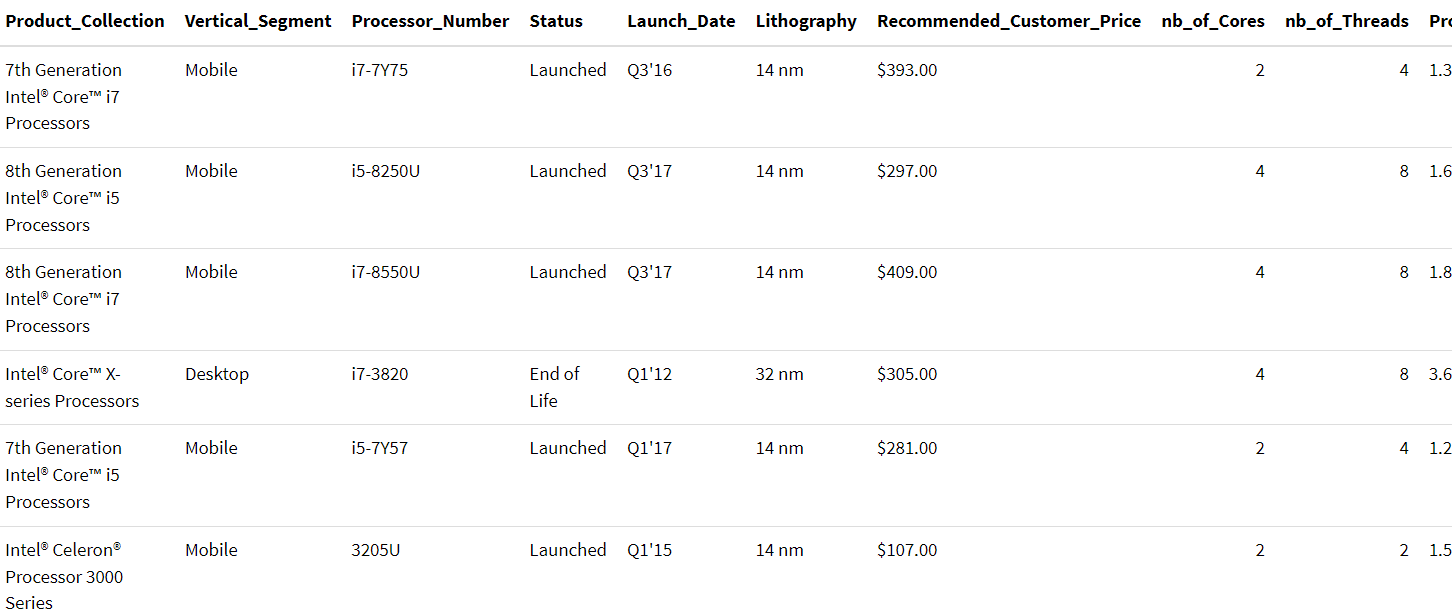
\includegraphics[width=\textwidth]{img/cpu-head.png}
  \vspace{0.5cm}
  \caption{First instances of CPUs data}
\end{figure}

Invalid cells may contain \texttt{NA}, an empty string, or other values showing us that this cell's data was not collecting correctly. At the very first step, we want to selected only columns whose the percentage of valid cells exceeds our predefined value. Then we filter out all instances with invalid features. Note that careful column selection possibly remains more instances for later tasks.

\begin{lstlisting}[caption={Cleaning functions}]
  # Check if a cell has a valid value
  is_valid <- function(value) {
    return(!is.na(value)
           & !is.null(value)
           & !value == ""
           & !value == "N/A"
           & !value == "-"
           & !value == "missing"
           & !value == "unknown")
    # Add your criteria
  }
  
  # Select columns with enough valid cells
  filtered_data <- function(data, valid_percentage=0.8) {
  selected_columns <- character(0) 
  
  for (col in colnames(data)) { 
    valid_count <- sum(is_valid(data[[col]])) 
    total_instances <- length(data[[col]]) 
    
    if ((valid_count / total_instances) >= fill) {
      selected_columns <- c(selected_columns, col)
    }
  }
  
  return(data[selected_columns])
}
  \end{lstlisting}


\begin{lstlisting}[caption={Cleaned data and selected features}]
  filtered_cpu_data <- filtered_data(cpu_data, 0.4)

  processed_cpu_data <- 
    filtered_cpu_data[
      apply(filtered_cpu_data, 1, function(row) all(sapply(row, is_valid))), ]
  
  selected_cpu_data <- processed_cpu_data[, c("Recommended_Customer_Price",
                                              "Product_Collection",
                                              "Launch_Date",
                                              "nb_of_Cores",
                                              "nb_of_Threads", 
                                              "Processor_Base_Frequency",
                                              "Bus_Speed")]
  
  # Adjust selected columns for your later needs

  kable(head(selected_cpu_data), format = "html") %>%
  kable_styling()
\end{lstlisting}

\begin{figure}[!ht]
  \centering
  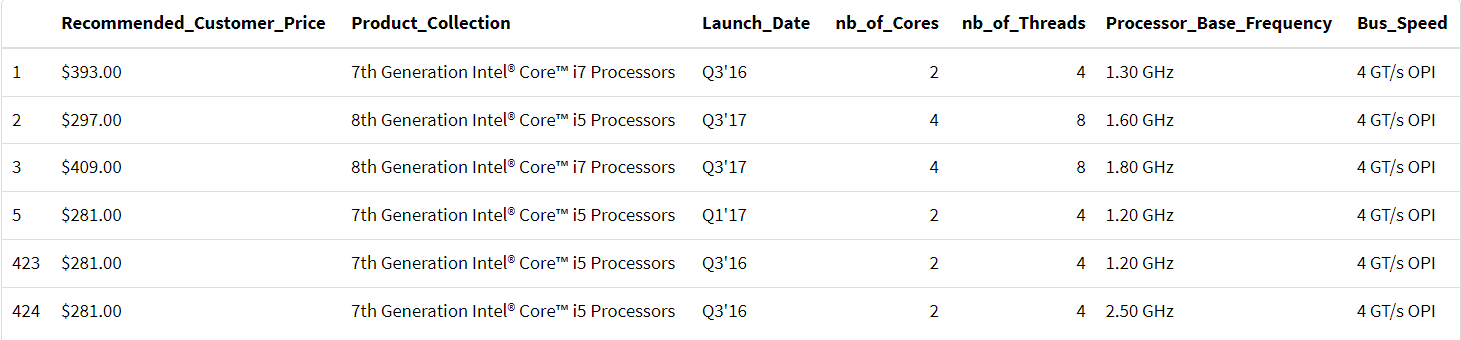
\includegraphics[width=\textwidth]{img/cpu-selected-head.png}
  \vspace{0.5cm}
  \caption{First instances of selected CPUs data}
\end{figure}

\section{Data Pre-computation}

Some features in our data have values that need to be reformatted for easily later sorting and analyses. Therefore, we need to gain a good understand on the features.


\begin{lstlisting}[caption={A processing for selected features}]
  cpu_columns <- colnames(cpu_data)
  gpu_columns <- colnames(gpu_data)
  intersect(cpu_columns, gpu_columns)
  # Output: character(0)
\end{lstlisting}

Since the data files have no common features, let us take a look at them independently.



\end{document}
